\documentclass{article}
\usepackage[utf8]{inputenc}
\usepackage[dutch]{babel}
\usepackage{url}
\usepackage[style=numeric,sorting=none,backend=bibtex]{biblatex}
\bibliography{biblatex_DAV.bib}


\title{Oorzaken en gevolgen van fluctuaties in voedselprijzen in niet-Westerse landen}
\author{Janne Spijkervet 10879609\\ Jardenna Mohazzab 11701145\\ Jonne Goedhart 11890169 \\Julius Huizing 11898402}
\date{\today{}}
\usepackage{graphicx} %package to manage images
\graphicspath{ {./images/} }
%Data Analysis and Visualization



\begin{document}


\maketitle

\newpage

\section*{Inleiding}
% Toen de VOC in de 16e eeuw kruiden en specerijen met de rest van de wereld begon te verhandelen werd een nieuw tijdperk ingeluid. Steeds meer landen volgden het Nederlandse voorbeeld en begonnen handel met elkaar te drijven. Zo ontstond langzaam maar zeker de huidige wereldmarkt waar de prijs van voedselproducten wordt bepaald vraag en aanbood over de gehele wereld.\\

De groei van de internationale handel heeft er voor gezorgd dat meer landen toegang hebben tot meer buitenlandse producten. Maar het zorgde ook voor meer afhankelijkheid tussen landen, zoals duidelijk werd tijdens de wereldwijde voedselcrisis van 2007. Van veel breed-geconsumeerde producten stegen de prijzen in korte tijd onvoorspelbaar hoog. Zo steeg de wereldwijde prijs van rijst binnen twee jaar met  217\% en de prijs van graan met 136\% \cite{steinberg2008financial}. Hoewel dit ook in ontwikkelde landen voor veel economische en sociale onrust zorgde, bleken hierdoor vooral de ontwikkelingslanden nog armer te worden \cite{ivanic2008implications}. \\

Er is veel onderzoek gedaan naar mogelijke oorzaken van prijsstijgingen, met als doel een herhaling van de voedselcrisis te voorkomen. Zo blijkt het toenemende gebruik van biobrandstoffen de voedselprijzen te verhogen. Immers kunnen gewassen die gebruikt worden voor de productie van brandstof niet meer worden gebruikt voor de productie van voedsel \cite{mitchell2008note}. 
Ook blijkt dat de olieprijs positief gecorreleerd is aan voedselprijzen, omdat het zowel de energiebron is voor mechanische voedselproductie als voor het transporteren ervan \cite{zubrin2008food}. Bovendien vergroot een stijging van de olieprijs weer de vraag naar biobrandstoffen.\\

% Hier wordt met behulp van verschillende data-sets getracht deze mogelijke oorzaken te bevestigen, wat leidt tot de volgende deelvragen:\\
% - Bestaat er een verband tussen de olieprijs en voedselprijzen? \\
% - Bestaat er een verband tussen het bio-brandstofgebruik en voedselprijzen? \\
% Er wordt een positieve correlatie verwacht tussen de olieprijs en alle voedselproducten. Dit is aannemelijk omdat vrijwel alle voedselproducten transport vereisen en hun prijzen daarom afhankelijk zijn van de olieprijs.
% Bovendien wordt verwacht dat de het bio-brandstofgebruik en de prijzen van mais positief gecorreleerd zijn, omdat mais één van de meest populaire gewassen voor bio-brandstof is [Bron]. \\

Naast brandstofgebruik en olieprijzen kunnen echter nog meer factoren in verband staan met fluctuaties van voedselprijzen, zoals geografische factoren. Daaruit volgt de volgende deelvraag: 
\textit{Vertonen landen in dezelfde regio’s vergelijkbare prijsverschillen?}
Er wordt verondersteld dat landen in dezelfde sub-regio's soortgelijke fluctuaties in voedselprijzen over dezelfde gewassen laten zien. Dit is aannemelijk omdat landen in dezelfde regio's een gelijksoortig klimaat kennen. Dit wordt onderzocht door met k-means landen te classificeren. Verwacht wordt dat het clusteren van landen binnen één regio geen vaste cluster-groepen oplevert.  \\
%En dat lange periodes van droogte leiden tot prijsstijgingen van producten zoals rijst en graan. \\

Daarnaast zijn voedselproducten te categoriseren en bestaan voedselproducten vaak uit andere voedselproducten.
Daarom wordt ook geprobeerd de volgende deelvragen te beantwoorden:
\textit{Zijn er voedselprijzen die positief of negatief aan elkaar gecorreleerd zijn?}\textit{Als voedselprijzen aan elkaar gecorreleerd zijn, is dit dan altijd het geval of alleen tijdens bepaalde periodes?}
Er wordt verondersteld dat producten uit dezelfde categorieën soortgelijke prijsfluctuaties laten zien, en dat de prijsfluctuatie van een voedselproduct dat uit meerdere ingrediënten bestaat, overeenkomt met de prijsfluctuaties van de individuele ingrediënten waaruit dat product bestaat. 
Dit wordt onderzocht door verschillende producten te classificeren met k-means. Daarna worden de correlaties tussen producten binnen een cluster met elkaar vergeleken.
Verwacht wordt dat producten uit dezelfde categorie samen geclusterd worden en dat correlatie tussen producten binnen deze clusters sterk is. Bovendien wordt verwacht dat de periode daar geen invloed op heeft.\\ 
\newpage
Ook worden voedselprijzen in verschillende valuta gegeven, maar deze valuta zijn niet allemaal even stabiel of gelijk in waarde. Dit leidt tot de volgende deelvraag:
\textit{Zijn de wisselkoersen gecorreleerd aan de productprijzen in een land?}
Er wordt verondersteld dat er een negatieve lineaire relatie is tussen de wisselkoers (USD per valuta) van een valuta en de prijs van producten. Dit is aannemelijk omdat als de valuta meer waard wordt het goedkoper voor bedrijven is om producten te importeren waardoor de prijzen kunnen dalen. 
Hier wordt dat onderzocht door de gemiddelde correlatie tussen alle productprijzen en wisselkoersen te bepalen.
Er wordt verwacht als de wisselkoers hoger wordt dat de prijs van dat product zal dalen.\\

Bovendien bestaan er vaak ook grote verschillen in welvaart tussen landen. Dat leidt tot de volgende deelvraag:
\textit{Geven prijzen gecorrigeerd op het Gross Domestic Product (GDP) een ander beeld dan prijzen in USD?}
Er wordt vanuit gegaan dat het GDP van een land niet gecorreleerd is met productprijzen.
Bovendien wordt verondersteld  dat corrigeren op GDP een betrouwbaarder beeld geeft van de betaalbaarheid van producten. Immers kan de GDP tussen landen erg verschillen. Hier wordt dat onderzocht door landen met k-means te classificeren op voedselprijzen in USD. Vervolgens worden alle landen opnieuw geclassificeerd, maar dan met prijzen gecorrigeerd op GDP. Verwacht wordt dat dit tot verschillende classificaties leidt.\\

%Hier wordt dat onderzocht door van verschillende landen de voedselprijzen in US-Dollar te bepalen, en deze landen met k-means te laten clusteren tot groepen die vergelijkbare prijzen hebben. Vervolgens is dit voor alle landen herhaald, maar dan met prijzen gecorrigeerd op GDP. Verwacht wordt dat landen met de GDP correctie anders geclusterd worden.\\

Tot slot wordt de beschikbaarheid van voedsel vaak in verband gebracht met gezondheid, daarom wordt ook geprobeerd de volgende deelvragen te beantwoorden: 
\textit{Bestaat er een verband tussen de voedselprijzen en het sterftecijfer in een land?}
\textit{Bestaat er een verband tussen vluchtelingen-stromingen en voedselprijzen?} 
Er wordt vanuit gegaan dat hoge voedselprijzen een negatieve invloed heeft op de algemene gezondheid in een land. Bovendien wordt verwacht dat hoge prijzen een stimulans voor emigratie kunnen zijn. Hier wordt dat onderzocht door voedselprijzen met sterfte- en vluchtelingen cijfers te vergelijken. Er wordt een positieve correlatie verwacht tussen vluchtelingenstromen, sterftecijfers en voedselprijzen. \\

Om deze deelvragen te kunnen beantwoorden is gebruik gemaakt van de Global Food Prices (GFP) Database  van het World Food Programma \cite{wfp}. In de database zijn voor 76 verschillende landen de maandelijkse voedselprijzen gegeven voor veel geconsumeerde voedselwaren zoals bonen, rijst en olie. Deze database wordt uitgebreid genormaliseerd zodat zowel de voedselprijzen van verschillende producten met elkaar vergeleken kunnen worden als de prijsveranderingen tussen landen en gebieden. \\

\newpage

\section*{Methode}

\subsection*{Pre-processing}
Ten eerste is het aantal kolommen van de dataset verminderd. De kolom met de provincies is verwijderd omdat bij het merendeel van de provincies enkel data was verzameld van één stad, waardoor deze kolom geen extra informatie bevatte dan de kolom met steden zelf (zie figuur \ref{fig_prov}). Ook waren in de oorspronkelijke dataset de jaren en de maanden gegeven in aparte kolommen. Deze zijn samengevoegd tot één kolom.\\

\begin{figure}[h!]
\centering
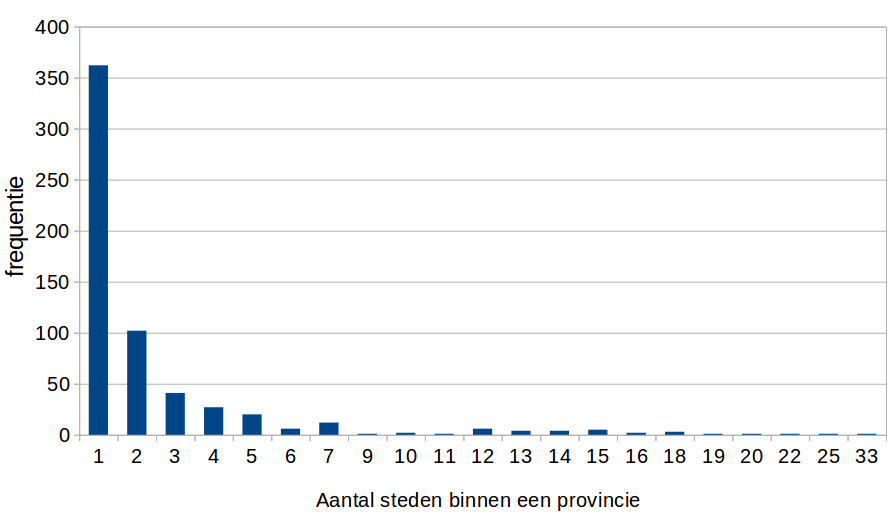
\includegraphics[scale=0.38]{provincie}
% deze caption later verbeteren
\caption{Het aantal provincies met hetzelfde aantal gedocumenteerde steden}
\label{fig_prov}
\medskip
\small 
In de GFP Database was bij veel provincies slechts data van één stad gedocumenteerd.
 \end{figure}

% Vervolgens zijn identieke stads-namen die bij verschillende landen hoorden gedisambigueerd door de afkorting van het betreffende land erachter te zetten. Zo werd San Vicente veranderd naar Sante Vicente (Sal).  Dit was wenselijk omdat er later bij de visualisatie per stad data opgevraagd zou worden.\\
 
In de database waren ook veel producten in verschillende eenheden gedocumenteerd. Zo was bijvoorbeeld de melkprijs zowel per 500 gram als per liter gegeven (zie figuur \ref{fig_milk}). Daarom zijn alle eenheden in de dataset genormaliseerd om het vergelijken van prijzen te vergemakkelijken. Daarvoor is handmatig een \textit{dictionary} aangemaakt met als \textit{keys} alle te converteren eenheden en met als \textit{values} de desbetreffende \textit{conversion rates}. Zo zijn de melkprijzen in liters gedeeld door de \textit{value} van liter in de \textit{dictionary}, waardoor alle melkprijzen nu in KG zijn gegeven. Op deze manier is ervoor gezorgd dat alle producten in een unieke eenheid vermeld staan. De \textit{conversion rates} zijn verkregen uit \textit{metrix conversion rates}\cite{conv} en \textit{density conversion rates}\cite{conversion}. Eenheden waarvoor geen \textit{conversion-rate} gevonden kon worden, zijn de betreffende rijen van verwijderd, zoals bij bijvoorbeeld de eenheden \textit{quartillas} en \textit{goat heads}.\\
 
\begin{figure}[h!]
\centering
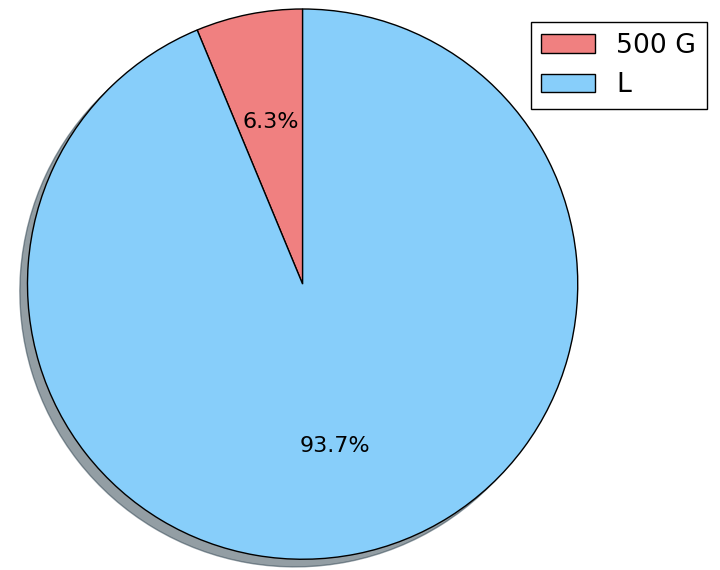
\includegraphics[scale=0.25]{milk}
\caption{De verdeling van melk eenheden voor normalisatie}
\label{fig_milk}
\medskip
\small 
Om voedselprijzen met elkaar te kunnen vergelijken, was het noodzakelijk alle voedselprijzen te normaliseren naar een unieke eenheid.

 \end{figure}

 
% Daarna zijn alle eenheden genormaliseerd om het vergelijken van prijzen te vergemakkelijken.
% Daarvoor zijn alle eenheden omgezet naar Kg of unit. Hiervoor is handmatig een \textit{dictionary} gemaakt met als \textit{keys} alle te converteren eenheden en met als \textit{values} de desbetreffende \textit{conversion rates}. Zo was de melkprijs zowel per liter als per \textit{gallon} gegeven. Om dit te normaliseren zijn de prijzen van \textit{gallon} gedeeld door de \textit{value} van \textit{gallon} in de \textit{dictionary}, namelijk 3.78541178. Om de \textit{conversion rates} te achterhalen is gebruik gemaakt van een online \textit{metric converter} \cite{conv} en een online \textit{density converter} \cite{conversion}. Marmite heeft geen vaste \textit{conversion-rate}, maar er wordt uitgegaan van 2.445 Kg per \textit{marmite} \cite{Marmite}. Eenheden waarvoor geen \textit{conversion-rate} gevonden kon worden zijn de betreffende rijen verwijderd, zoals bij bijvoorbeeld de eenheden \textit{quartillas} en \textit{goat heads}.\\

Bovendien is voor elk land in de database de voedselprijs in verschillende wisselkoersen gedocumenteerd. Om prijzen tussen landen te vergelijken was het daarom noodzakelijk alle prijzen te normaliseren naar één wisselkoers. Hier is ervoor gekozen alle prijzen naar US-Dollar (USD) te normaliseren, omdat de USD één van de meest stabiele wisselkoersen is. Hiervoor is gebruik gemaakt van een historische database van de wisselkoersen \cite{curr_rate}. Rijen met valuta 's waarvoor geen officiële wisselkoers kon worden gevonden zijn verwijderd. Zo bleek de bijvoorbeeld \textit{Somaliland Shilling} (SOS)  geen officieel erkende munteenheid te zijn en was er voor de \textit{Armenian Dram} (AMD) pas wisselkoers-informatie beschikbaar vanaf februari 2003. Zo zijn alle rijen waar de prijs in SOS was gegeven verwijderd, en alle rijen vóór februari 2003 waar de prijs in AMD gegeven was ook.\\

Om een beter beeld van de betaalbaarheid van producten binnen een land te krijgen, is er een nieuwe maatstaf berekend die rekening houdt met de koopkracht van een land. Hiervoor is gebruik gemaakt van een historische database met GDP's \textit{per capita} \cite{GDP}. 
Door telkens de GDP van een land te delen door de prijs van een product in dat land, ontstaat een getal dat aangeeft hoeveel er van dat product in het desbetreffende land gekocht kan worden. Dat getal wordt de 'betaalbaarheid-index' genoemd. Hoe hoger de betaalbaarheid-index van een product in een land, hoe betaalbaarder dat product is voor de inwoners van dat land.\\ % voorbeeld?

% Omdat nu alle prijzen naar USD waren omgezet, was het ook mogelijk prijzen per land te normaliseren op \textit{gross domestic product} (GDP). Hiervoor is gebruik gemaakt van een historische database met GDP's \textit{per capita} wereldwijd \cite{GDP}. Door telkens de GDP's van landen door de prijzen van producten in dat land te delen, ontstaat een maat die aangeeft hoeveel er van dat product in het betreffende land gekocht kan worden. Dat getal wordt de 'betaalbaarheid-index' genoemd. Hoe hoger de betaalbaarheid-index van een product in een land, hoe betaalbaarder dat product voor de inwoners van dat land is. \\

Om voedselprijzen over de tijd met elkaar te vergelijken, is het bovendien noodzakelijk om voor elk product over lange periodes aan onafgebroken voedselprijzen te beschikken. In de dataset zaten echter veel tijds-kloven in de documentatie van voedselprijzen. Kloven van één of twee maanden zijn daarom ingevuld met lineaire regressie. Als er na de toepassing van deze lineaire regressie nog steeds data-reeksen waren van minder dan zes maanden zijn deze reeksen verwijderd. Tenslotte zijn alle producten verwijderd waarvan minder dan één jaar aan data gedocumenteerd is.\\

% Om in staat te zijn verschillende voedsel prijs ontwikkelingen door de tijd met elkaar te vergelijken is het noodzakelijk om voor langere periodes aaneengesloten data te hebben. Dit is nodig, omdat lossen punten geen beeld geven van de ontwikkeling van de prijs stijging of daling. Om aaneengesloten data te krijgen zijn gaten van één of twee maanden opgevuld met lineaire regressie. Verder zijn data reeksen van minder dan 6 maanden verwijderd en moet er van een product minimaal één jaar aan data zijn.

Nu alle voedselprijzen over langere periode's met elkaar vergeleken kunnen worden, is voor elke productprijs nog de afgeleide bepaald zodat de daadwerkelijke veranderingen in voedselprijzen vergeleken kunnen worden. En is elk land ingedeeld in sub-regio’s zodat ook de voedselprijzen tussen gebieden vergeleken kunnen worden. Hiervoor is gebruik gemaakt van een samengestelde database met alle landen en sub-regio's \cite{region1, region2}. 

\subsection*{Algoritmes}

\subsubsection*{k-means Algoritme}
Omdat er verschillende product-prijzen over de tijd met elkaar vergeleken moeten worden, maar niet elk product over dezelfde tijdspan is gedocumenteerd, is het standaard k-means algoritme van \textit{scikit-learn} onbruikbaar. Er ontstaan dan immers \textit{NaN-values} op de tijdstippen waar het ene product wel is gedocumenteerd maar het andere product niet (zie figuur \ref{fig_Nans}). Daarom is er een aangepaste versie van het k-means algoritme geïmplementeerd die deze \textit{NaN-Values} niet meeneemt in de berekeningen. Verder werkt het algoritme op de standaard manier. Dat wil zeggen dat er op willekeurige plekken een door de gebruiker aantal clusters-centra worden geïnitieerd. Vervolgens wordt van elk data-punt de euclidische afstand tot de verschillende centra berekend en worden alle data-punten tot het dichtstbijzijnde cluster-centrum geclassificeerd. Dan wordt het gemiddelde van elk cluster berekend en worden de cluster-centra opnieuw geïnitieerd op dat gemiddelde. Tot slot worden alle data-punten opnieuw tot het dichtstbijzijnde cluster-centrum geclassificeerd. Dit proces wordt iteratief herhaald tot de totale afstand tussen alle data-punten en hun cluster-centra niet of nauwelijks meer afneemt, met een maximum van 100 iteraties. \\

\begin{figure}[h!]
\centering
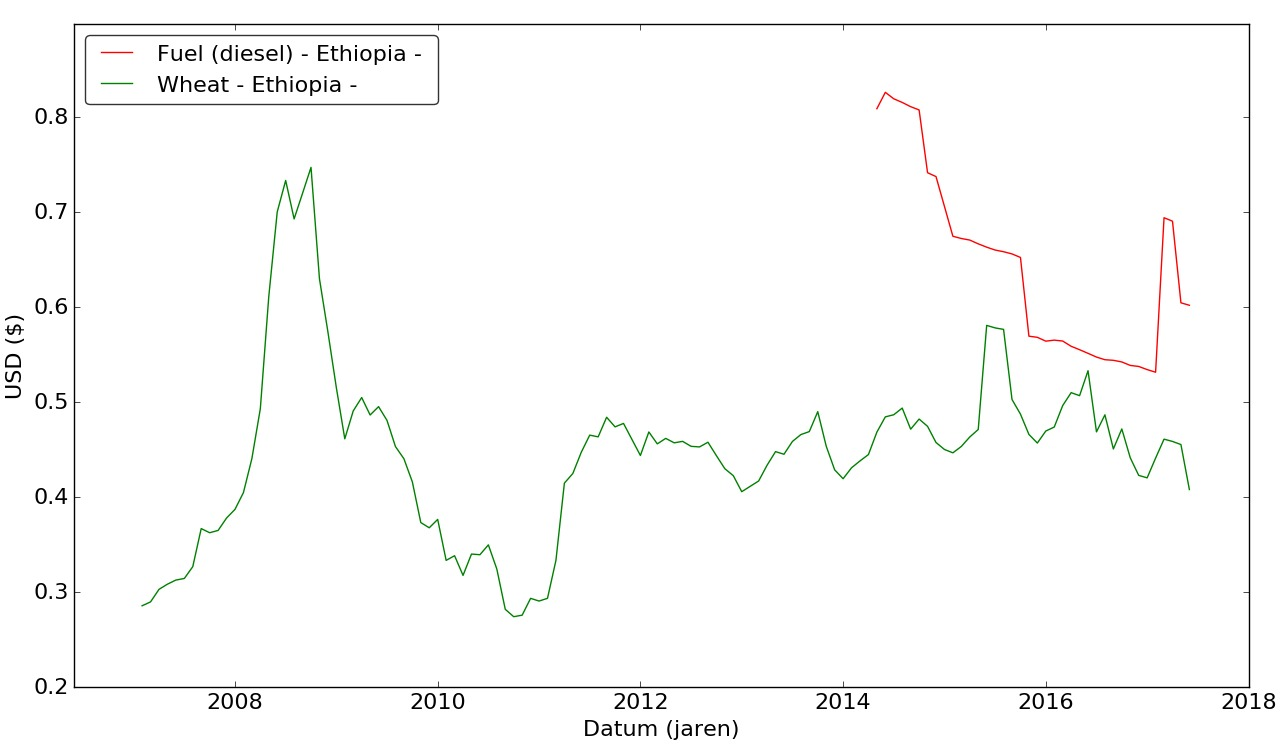
\includegraphics[scale=0.25]{EDA_K_means}
\caption{Het ontstaan van \textit{NaN-values} bij het vergelijken van prijzen }
\label{fig_Nans}
\medskip
\small
Wanneer voedselprijzen over verschillende tijdspannen zijn gedocumenteerd, wordt het k-means algoritme van \textit{scikit-learn} onbruikbaar. \end{figure}

Omdat k-means tot lokale-minima kan leiden, wordt in dit onderzoek k-means telkens met dezelfde parameters tien keer herhaald. Verder omdat k-means een \textit{unsupervised learning} algoritme is, wordt het hele proces herhaald met een verschillend aantal groepen. Hierna worden producten die in elke uitkomst van het k-means algoritme hetzelfde worden geclassificeerd als cluster beschouwd.

% \subsubsection*{T-SNE}
% Voor het visualiseren van de clusters is gebruik gemaakt van t-SNE. Dit is een techniek waarmee \textit{high-dimensional vectors} in een lijst van \textit{high-dimensional vectors} getransformeerd kan worden maar wel zodat de relatieve gelijkheid even groot blijft. Dit is dus een goede manier om \textit{high-dimensional data} te visualiseren en een goed overzicht te krijgen van de data. 

\subsubsection*{Karl-Pearson correlatie}
Om de correlatie tussen verschillende voedselprijzen te bepalen is tenslotte gebruik gemaakt van de Karl-Pearson correlatie coëfficiënt.
Dit algoritme geeft een getal terug die de sterkte van de lineaire samenhang tussen twee prijzen aangeeft. Daarbij houdt 1 een perfect lineair verband in en -1 een perfect negatief lineair verband in. Hiermee kan vervolgens worden afgeleid of twee producten afhankelijk zijn van dezelfde factoren of van elkaar.


\subsection*{Procedure}

\subsubsection*{Vertonen landen in dezelfde regio’s vergelijkbare prijsverschillen?}
Om landen binnen een regio goed met elkaar te kunnen vergelijken, moeten er zoveel mogelijk prijsvergelijkingen tussen die landen gemaakt worden. Daarom is gekeken naar de \textit{Sub-Saharan African}, omdat dit de regio is met het grootste aantal gedocumenteerde landen (zie figuur \ref{fig_sub-regio}). Tussen deze landen zijn vervolgens de kafferkoor (een alternatief voor mais) en de rijst prijzen vergeleken, omdat dit twee van de meest gedocumenteerde producten zijn (zie figuur \ref{fig_land_prod}). 
Vervolgens is geprobeerd de landen te classificeren met k-means, waarna binnen de clusters de correlatiecoëfficiënt tussen de landen is berekend.

%Deze producten zijn vervolgens door middel van k-means geclassificeerd. Tot slot is de correlatie tussen

\begin{figure}[ht!]
\centering
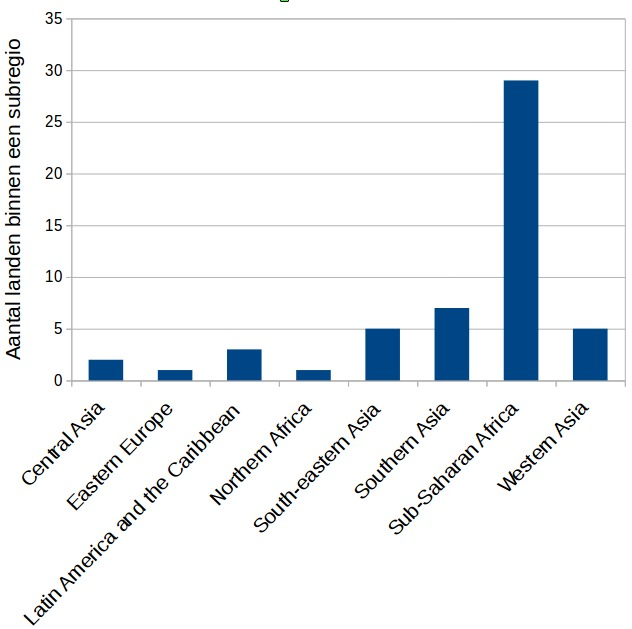
\includegraphics[scale=0.38]{EDA_1}
\caption{Het aantal landen per sub-regio }
\label{fig_sub-regio}
\medskip
\small
De Sub-Sahara blijkt het meeste landen over te hebben na pre-processing.  
\end{figure}

\begin{figure}[h!]
\centering
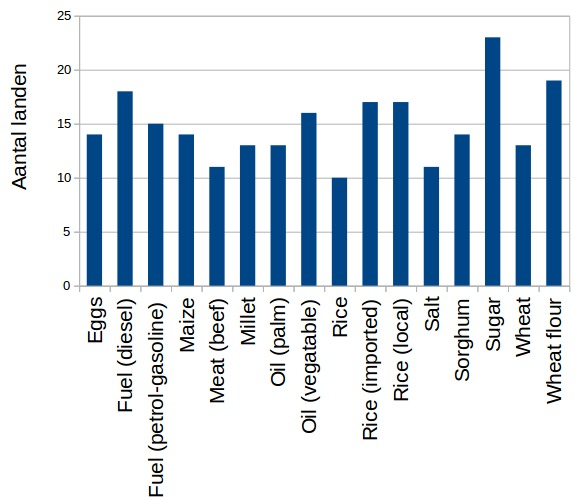
\includegraphics[scale=0.4]{EDA_2}
\caption{Het aantal landen per product}
\label{fig_land_prod}
\medskip
\small
\end{figure}

\subsubsection*{Zijn er voedselprijzen die positief of negatief aan elkaar gecorreleerd zijn? Als voedselprijzen aan elkaar gecorreleerd zijn, is dit dan altijd het geval of alleen tijdens bepaalde periodes?}
%Om te onderzoeken of er een verband bestaat tussen voedselprijzen is zoals eerder genoemd gefocust op de ingrediënten van producten. 
% Over Oekraïne tussen 2014 en 2018 was data beschikbaar van veel soorten vlees, vandaar dat dit land is gekozen om te onderzoeken voor deze deelvraag. Eerst zijn de genormaliseerde prijzen van alle producten in Oekraïne opgehaald en met behulp van bokeh geplot om een overzicht te krijgen van de relatieve veranderingen.
Om correlaties tussen voedselprijzen te bepalen, zijn er lange onafgebroken periodes aan voedselprijzen nodig.
Daarom is er naar de voedselprijzen in Oekraïne gekeken, omdat daar een groot aantal voedselproducten over dezelfde periode (2014-2018) zijn gedocumenteerd. Vervolgens zijn met k-means alle producten geclassificeerd, waarna binnen elk cluster de correlatiecoëfficiënt tussen de producten is berekend. Tot slot is gekeken of de classificaties en correlaties veranderen als er naar de periode 2014-2018 wordt gekeken.

\subsubsection*{Zijn de wisselkoersen gecorreleerd aan de productprijzen in een land?}
Hiervoor is voor elk land de correlatie bepaald tussen de productprijzen en de wisselkoers van dat land. 
Vervolgens is het gemiddelde van deze correlatie coëfficiënten berekend, waarvan ook de standaard afwijking is berekend.

% \subsubsection*{Is er een correlatie tussen de GDP en productprijzen van een land?}
% Hiervoor is voor elk land de correlatie bepaald tussen het GDP van dat land en de productprijzen.
% Vervolgens is het gemiddelde van deze correlatie coëfficiënten berekend, waarvan ook de standaard afwijking is berekend.



\subsubsection*{Geven prijzen gecorrigeerd op het Gross Domestic Product (GDP) een ander beeld dan prijzen in USD?}
Eerst is de correlatie tussen GDP en voedselprijzen berekend om te achterhalen hoe betrouwbaar de betaalbaarheid-index is als maatstaf. Als deze correlatie laag is kan de betaalbaarheid-index als zuivere maatstaf worden gebruikt. 
Vervolgens is naar de graanprijzen gekeken, omdat graan één van de meest-gedocumenteerde producten in de dataset is (zie figuur \ref{fig_land_prod}), waardoor er zoveel mogelijk landen met elkaar vergeleken kunnen worden.
Eerst zijn de graanprijzen in USD van alle landen in de dataset opgehaald, en zijn de landen op basis daarvan geclassificeerd. Hiervoor is gebruik gemaakt van het k-means algoritme. Vervolgens is de betaalbaarheid-index van graan voor elk land opgehaald en zijn op basis van deze index opnieuw alle landen in clusters ingedeeld. Om te kijken of de prijzen gecorrigeerd met GDP een andere beeld geven wordt er gekeken of clusters van landen uit dezelfde regio leiden tot verschillende classificaties.


\subsubsection*{Bestaat er een verband tussen de voedselprijzen en het sterftecijfer in een land?}

Om een verband tussen voedselprijzen en sterftecijfers te bepalen, is het wenselijk om de cijfers van landen te vergelijken waar sterftecijfers gelijkmatig verlopen. Immers als er een correlatie is tussen de sterftecijfers en voedselprijzen, kunnen de sterftecijfers niet leiden tot sterke fluctuaties in de voedselprijzen. Daarom zijn de voedsel- en sterftecijfers binnen Afghanistan en Niger vergeleken, omdat beide landen gelijkmatige verlopen in sterftecijfers vertonen (zie figuur \ref{fig_sterfte}). Vervolgens zijn de grafieken van de voedselprijzen en de sterftecijfers van beide landen vergeleken. Tot slot zijn voor beide landen ook de correlatiecoëfficiënten tussen beide cijfers berekend.

\subsubsection*{Bestaat er een verband tussen vluchtelingen-stromingen en voedselprijzen?}
Om een verband tussen voedselprijzen en vluchtelingen-stromingen te bepalen, is het wenselijk om de cijfers van landen te vergelijken waarbij grote stijgingen van vluchtelingen-cijfers te vinden zijn. Immers kan dan worden gekeken of deze stijgingen samen vallen met stijgingen in voedselprijzen. Daarom is gekeken naar Afghanistan en Georgië, omdat hier grote vluchtelingenstromen te vinden zijn.
In beide landen zijn de voedselprijzen en vluchtelingen-cijfers met elkaar vergeleken (zie figuur \ref{fig_ref_afg} en \ref{fig_ref_geor}). Tot slot zijn ook de correlatiecoëfficiënten tussen beide cijfers berekend.

\newpage
\section*{Resultaten}

\subsubsection*{Vertonen landen in dezelfde regio’s vergelijkbare prijsverschillen?}
Het k-means algoritme clustert de landen telkens in andere groepen.
Ook na het herhaald toepassen van het k-means algoritme komen er geen vaste cluster-groepen naar voren. 
De rijst en kafferkoor prijzen van alle landen lijken gelijksoortige fluctuaties door te maken (zie figuur \ref{rice-regio} en \ref{sorghum-regio}).
Op Ethiopië en Nigeria na, zijn de correlatiecoëfficiënten van de prijzen tussen alle landen aanzienlijk hoog (zie figuur \ref{rice-corr} en \ref{sorghum-corr}).


 \begin{figure}[h!]
        \centering
        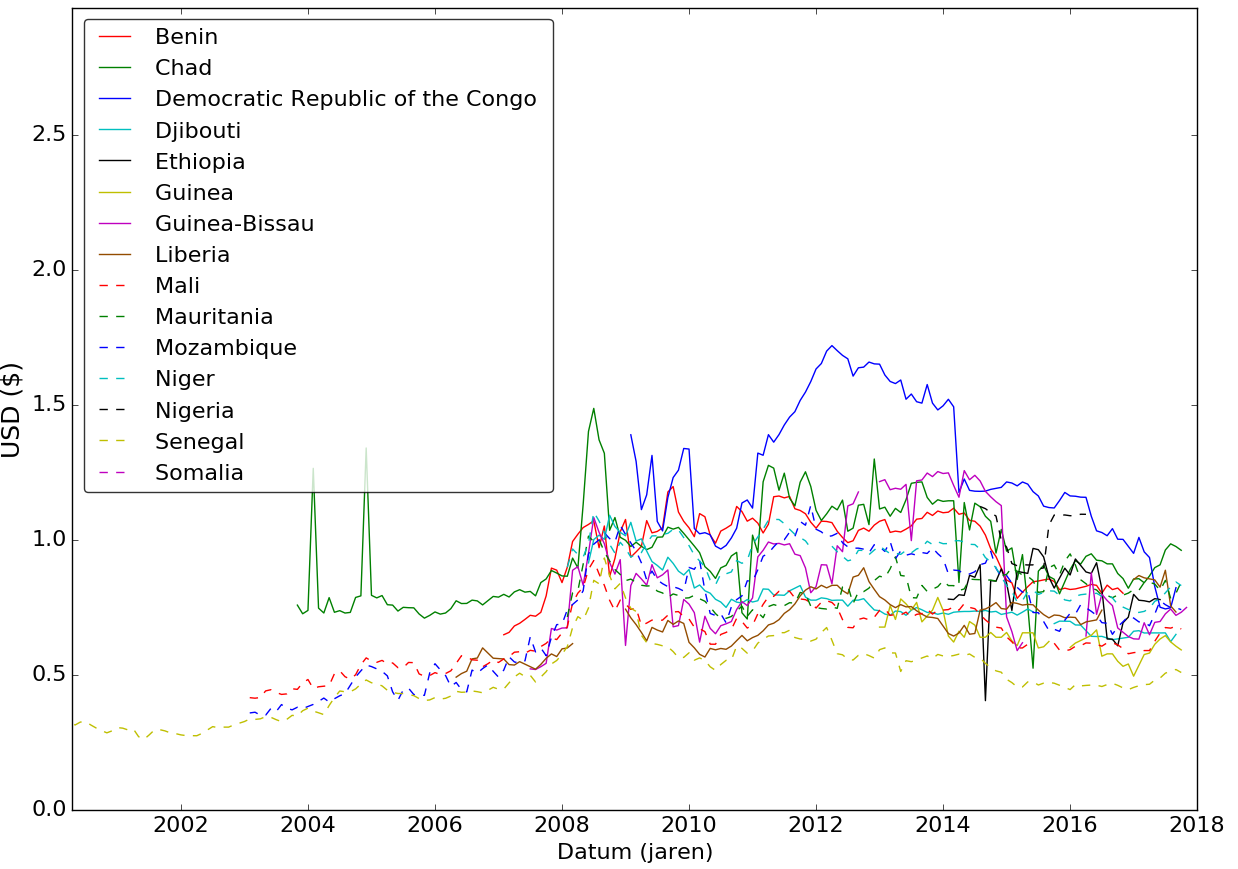
\includegraphics[scale=0.30]{rice.png}
        \caption{De prijs fluctuaties van rijst in de landen die behoren tot de \textit{Sub-Saharan Africa}.}
        \label{rice-regio}
        \medskip
        \small
        %India, Pakistan en Nepal door het k-means algoritme geclassificeerd tot het cluster met relatief goedkopere graanprijzen.  
        \end{figure}

 \begin{figure}[h!]
        \centering
        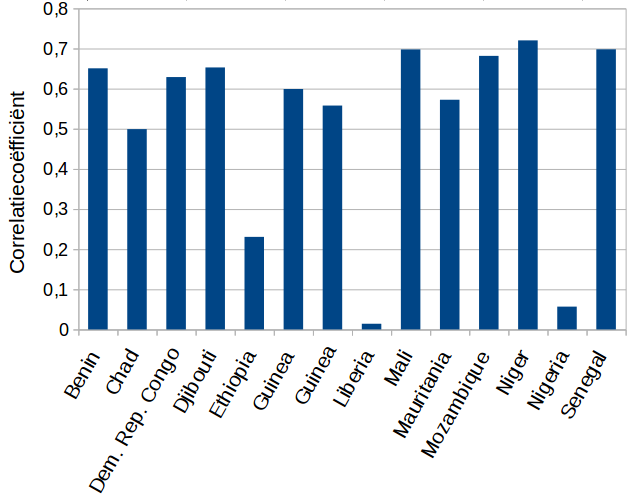
\includegraphics[scale=0.4]{rice_corr.png}
        \caption{De gemiddelde onderlinge correlatiecoëfficiënten tussen de rijst-prijzen van alle landen in de \textit{Sub-Saharan Africa} }
        \label{rice-corr}
        \medskip
        \small
        Op Ethiopië, Liberia en Nigeria na, vertonen alle landen binnen de \textit{Sub-Saharan Africa} sterke prijs correlaties met elkaar. 
        \end{figure}
        
 \begin{figure}[h!]
        \centering
        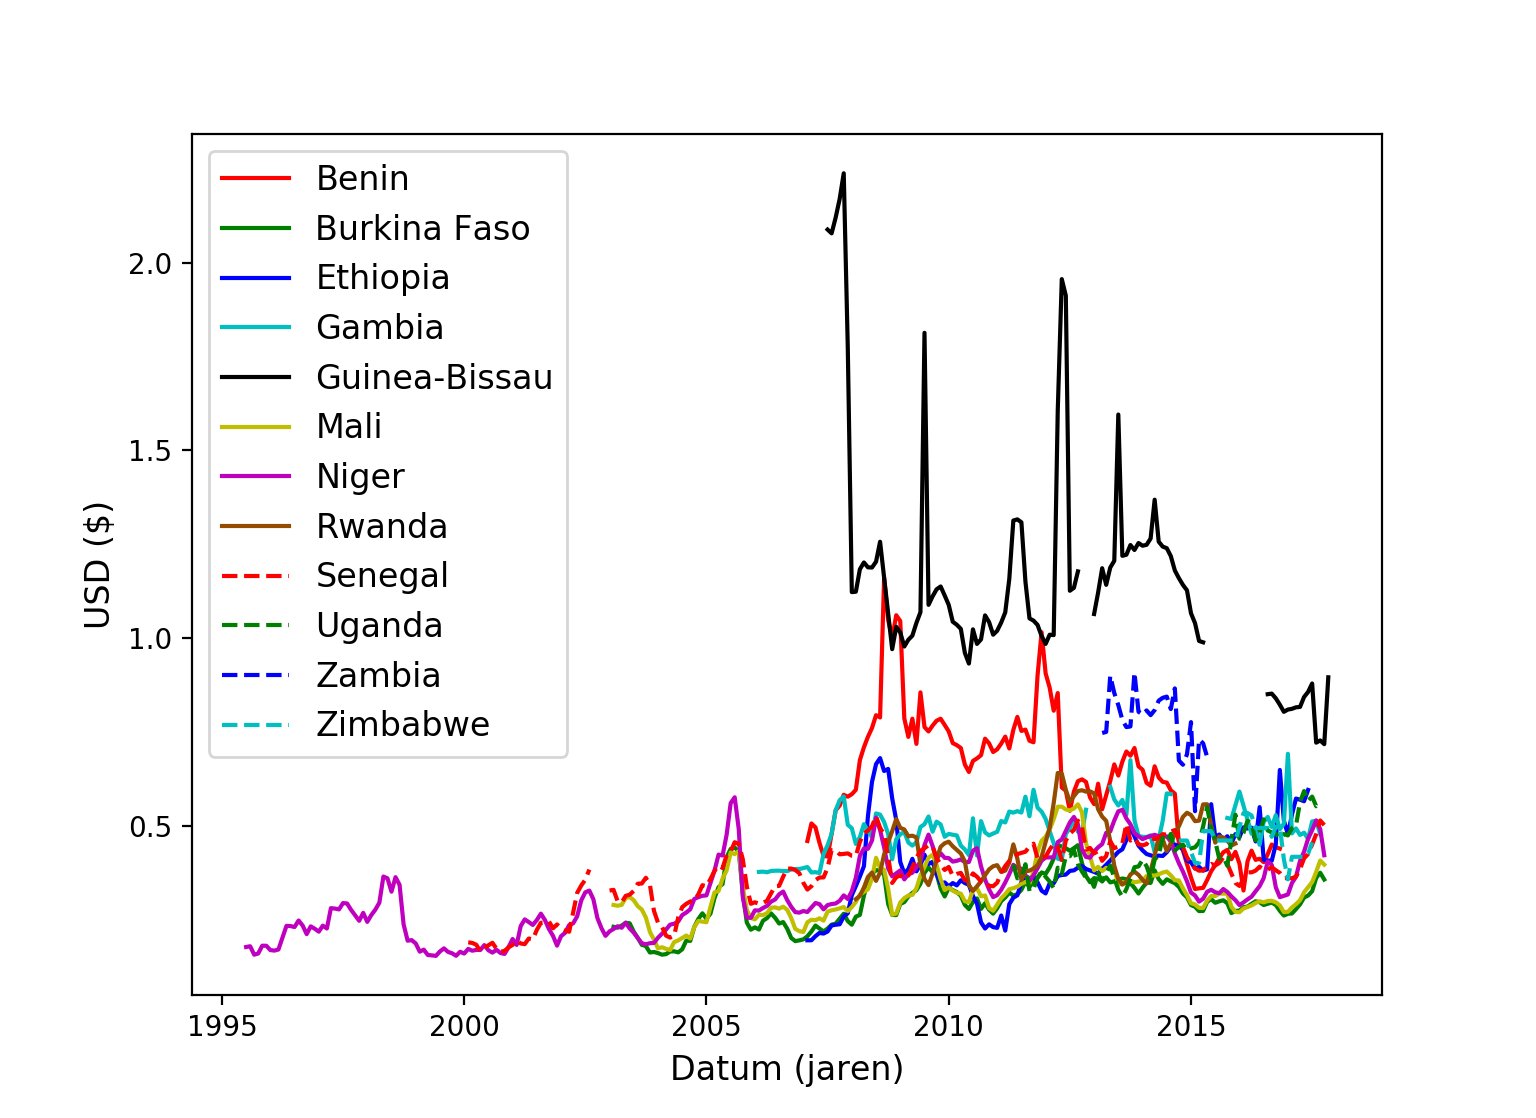
\includegraphics[scale=0.5]{sorghum.png}
        \caption{De prijs fluctuaties van kafferkoor in de landen die behoren tot Sub-Saharan Africa.}
        \label{sorghum-regio}
        \medskip
        \small
        %India, Pakistan en Nepal door het k-means algoritme geclassificeerd tot het cluster met relatief goedkopere graanprijzen.  
        \end{figure}

 \begin{figure}[h!]
        \centering
        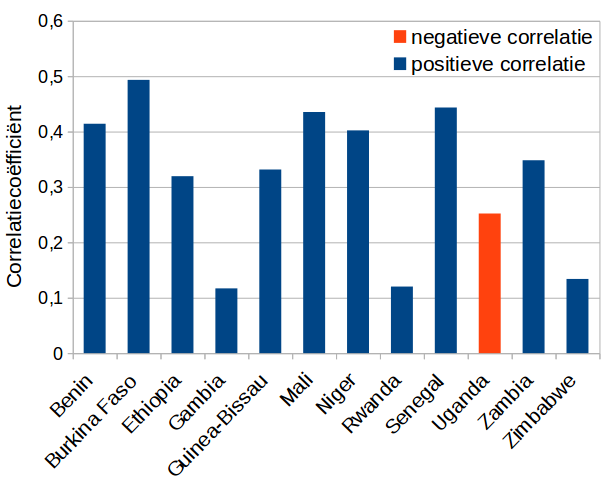
\includegraphics[scale=0.4]{sorghum_corr.png}
        \caption{De gemiddelde onderlinge correlatiecoëfficiënten tussen de kafferkoor-prijzen van alle landen in de in de \textit{Sub-Saharan Africa}}
        \label{sorghum-corr}
        \medskip
        \small
        De kafferkoor-prijzen van de verschillende landen in \textit{Sub-Saharan Africa} vertonen minder correlatie dan de rijst-prijzen.
        \end{figure}
\newpage

\subsubsection*{Zijn er voedselprijzen die positief of negatief aan elkaar gecorreleerd zijn? Als voedselprijzen aan elkaar gecorreleerd zijn, is dit dan altijd het geval of alleen tijdens bepaalde periodes?}
Over de periode 2013-2018 komt k-means tot zes clusters (zie tabel \ref{clusters-2013-2018}). Zo worden alle vleesproducten altijd samen in een cluster geplaatst en alle zuivelproducten ook. De prijzen van de producten binnen deze twee clusters correleren sterk (zie tabel \ref{zuivel-2014-2018} en \ref{vlees-2014-2018}), ook als de periode wordt gehalveerd (zie tabel \ref{zuivel-2014-2016} en \ref{vlees-2014-2016}).
 
 
 \begin{table}[ht!]
\centering
\caption{Correlaties tussen zuivel producten in Oekraïne tussen 2014 en 2018}
\label{zuivel-2014-2018}
\begin{tabular}{l|lll}
            & Butter   & Milk     & Sour cream \\ \hline
Milk        & 0.975480 &          &            \\
Sour cream  & 0.977874 & 0.996946 &            \\
Curd        & 0.864318 & 0.930772 & 0.931195  
\end{tabular}
\end{table}

 \begin{table}[ht!]
\centering
\caption{Correlaties tussen zuivel producten in Oekraïne tussen 2014 en 2016}
\label{zuivel-2014-2016}
\begin{tabular}{l|lll}
            & Butter   & Milk     & Sour cream \\ \hline
Milk        & 0.989415 &          &            \\
Sour cream  & 0.994624 & 0.997019 &            \\
Curd        & 0.985668 & 0.990619 & 0.994061  
\end{tabular}
\end{table}


\begin{table}[h!]
\centering
\caption{Correlaties tussen de prijs van vlees producten in Oekraïne tussen 2014 en 2018}
\label{vlees-2014-2018}
\begin{tabular}{l|lll}
                      & Meat (chicken, whole) & Meat (mixed, sausage) & Meat (pork) \\ \hline
Meat (mixed, sausage) & 0.968654              &                       &             \\
Meat (pork)           & 0.943341              & 0.957977              &             \\
Meat (beef)           & 0.946048              & 0.962734              & 0.981646   
\end{tabular}
\end{table}

\begin{table}[h!]
\centering
\caption{Correlaties tussen de prijs van vlees producten in Oekraïne tussen 2014 en 2016}
\label{vlees-2014-2016}
\begin{tabular}{l|lll}
                      & Meat (chicken, whole) & Meat (mixed, sausage) & Meat (pork) \\ \hline
Meat (mixed, sausage) & 0.956601              &                       &             \\
Meat (pork)           & 0.935190              & 0.957254              &             \\
Meat (beef)           & 0.955861              & 0.953394              & 0.969657   
\end{tabular}
\end{table}


\begin{table}[h!]
\centering
\caption{Clusters voor de producten van Oekraïne tussen 2013 en 2018 }
\label{clusters-2013-2018}
\begin{tabular}{l|lllll}
cluster 1 & Butter & Curd & Milk & Sour & \\
cluster 2 & Meat (beef) & Meat (chicken, whole) & Meat (mixed, sausage) & Meat (pork) & \\
cluster 3 & Fuel (diesel) & Fuel (petrol-gasoline) & & & \\
cluster 4 & Cabbage       & Carrots                & Onions                & Potatoes    &                           \\
cluster 5 & Eggs & Pasta & Rice & Sugar       & Wheat flour (first grade) \\
cluster 6 & Bread (rye)   & Bread (wheat)          & Oil (sunflower)       &             &                           \\ \hline
overige   & Beetroots     & Fat (salo)             & Buckwheat grits       &             &                          
\end{tabular}
\end{table}

\subsubsection*{Zijn de wisselkoersen gecorreleerd aan de productprijzen in een land?}
De gemiddelde correlatie tussen de productprijzen en de wisselkoers van een land is -0.282759847357, met een standaardafwijking van 0.44391608611.


\subsubsection*{Geven prijzen gecorrigeerd op het Gross Domestic Product (GDP) een ander beeld dan prijzen in USD?}
India, Pakistan, Nepal en Afghanistan blijken nabijgelegen landen te zijn die met beide maatstaven verschillend worden geclassificeerd. 
Met de graanprijzen in USD vertonen India, Pakistan en Nepal gelijksoortige graanprijzen. Deze drie landen worden door k-means dan ook samen geclassificeerd tot het cluster met relatief goedkope graanprijzen. Afghanistan wordt daarentegen geclassificeerd tot het cluster met relatief dure graanprijzen. Echter, wanneer er wordt gekeken naar de betaalbaarheid-index, verandert vooral de betaalbaarheid van graan in Nepal aanzienlijk. Zo wordt Nepal nu samen met Afghanistan tot het cluster met relatief dure graanprijzen geclassificeerd. Bovendien is de gemiddelde correlatie tussen GDP en productprijzen -0.0241052410847, met een standaardafwijking van 0.476439983355.
 
 
        \begin{figure}[ht!]
        \centering
        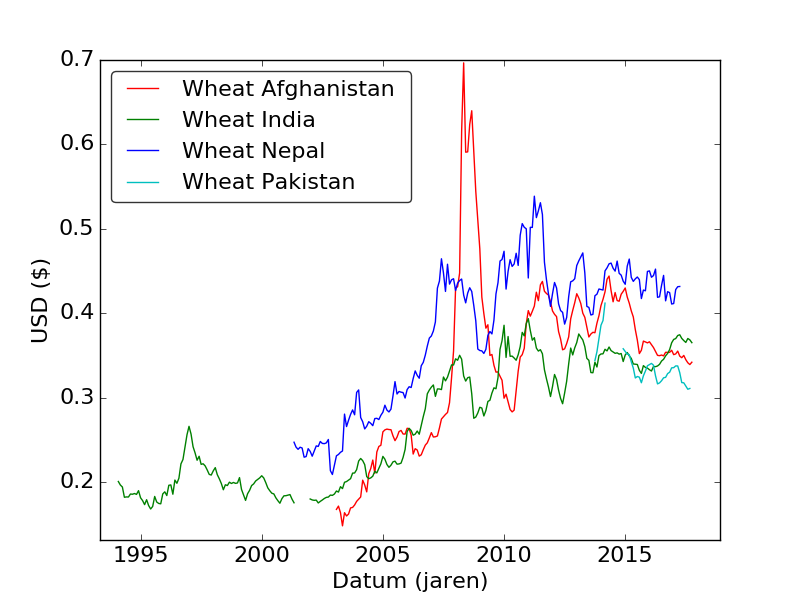
\includegraphics[scale=0.42]{images/wheat_vs4.png}
        \caption{De betaalbaarheid van graan in US-Dollars}
        \medskip
        \small
        India, Pakistan en Nepal worden door k-means geclassificeerd tot het cluster met relatief goedkope graanprijzen, terwijl Afghanistan wordt geclassificeerd tot het cluster met relatief dure graanprijzen.
        \end{figure}
        
        \begin{figure}[ht!]
        \centering
        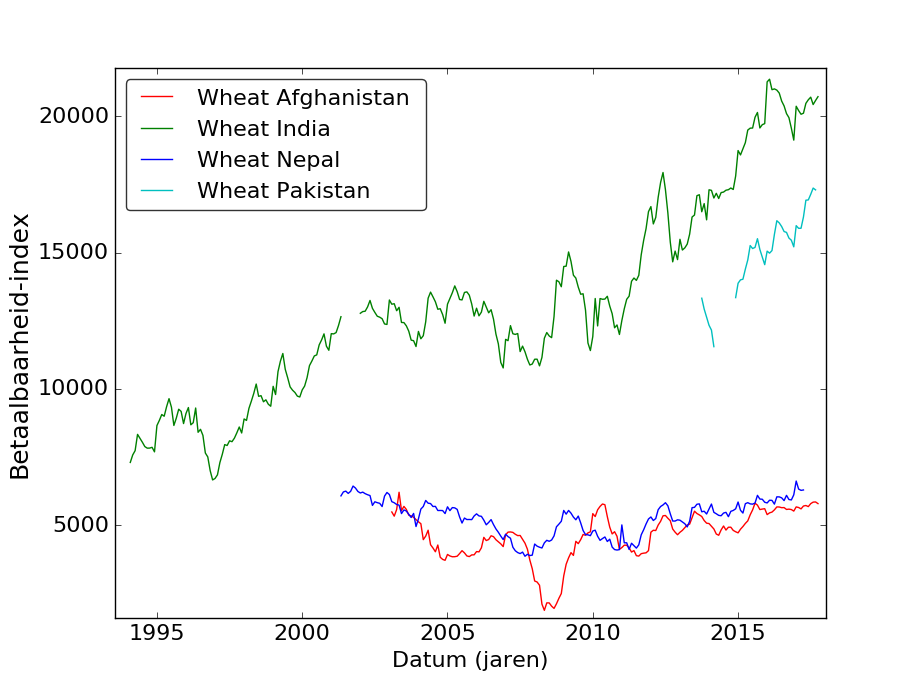
\includegraphics[scale=0.42]{images/wheat_vs5.png}
        \caption{De betaalbaarheid van graan zoals gegeven door de betaalbaarheid-index}
        \medskip
        \small
        Als er wordt gekeken naar de betaalbaarheid-index, wordt Nepal samen met Afghanistan geclassificeerd tot het cluster met relatief dure graanprijzen.
        \end{figure}
        
        
 
% \begin{figure}[h!]
 %       \centering
  %      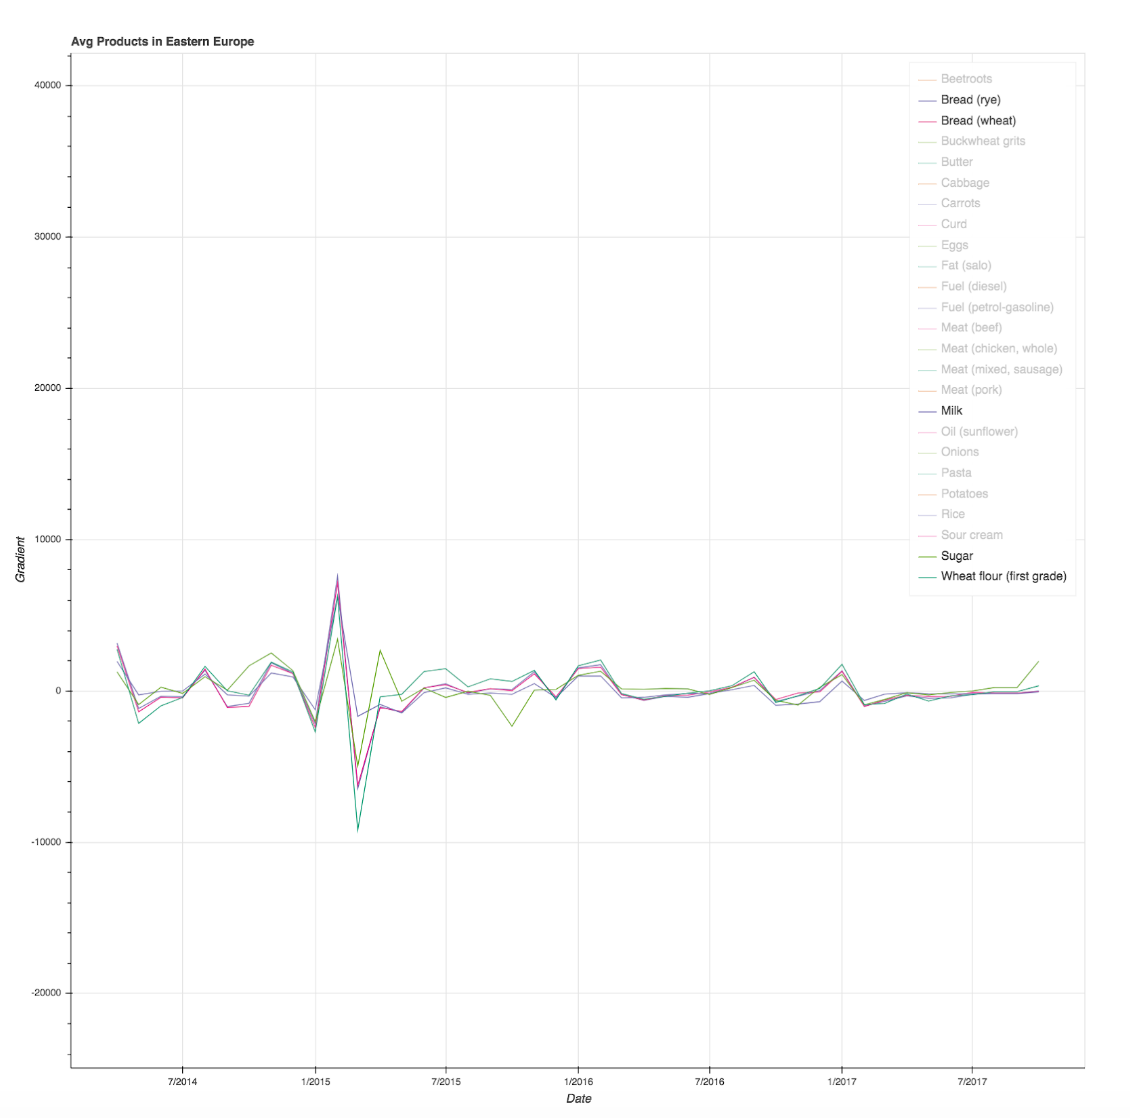
\includegraphics[scale=0.7]{oekraine.png}
   %     \caption{De afnames en toenames in de prijs van de ingrediënten van brood in Oekraïne geplot over een periode van ongeveer 2013 tot 2018.}
    %    \medskip
     %   \small
      %  %India, Pakistan en Nepal door het k-means algoritme geclassificeerd tot het %cluster met relatief goedkopere graanprijzen.  
       % \end{figure}

%grafiek naam moet veranderd worden naar Oekraïne


 
 
 
 


%grafiek naam moet veranderd worden naar Oekraïne

\newpage
\subsubsection*{Bestaat er een verband tussen de voedselprijzen en het sterftecijfer in een land?}
Zoals verwacht verlopen de sterftecijfers van Afghanistan en Niger gelijkmatig (zie figuur \ref{fig_sterfte}) in de periode 2000 en 2015.
De voedselprijzen in beide landen fluctueren echter onregelmatig tussen 2004 en 2014 (zie figuur \ref{mortality_afghanistan} en \ref{mortality_niger}). De gemiddelde correlatie van de voedselprijzen in Afghanistan en het sterftecijfer tussen 2004 en 2014 is -0.73. Voor Niger is die correlatie -0.24.

\begin{figure}[h!]
    \centering
    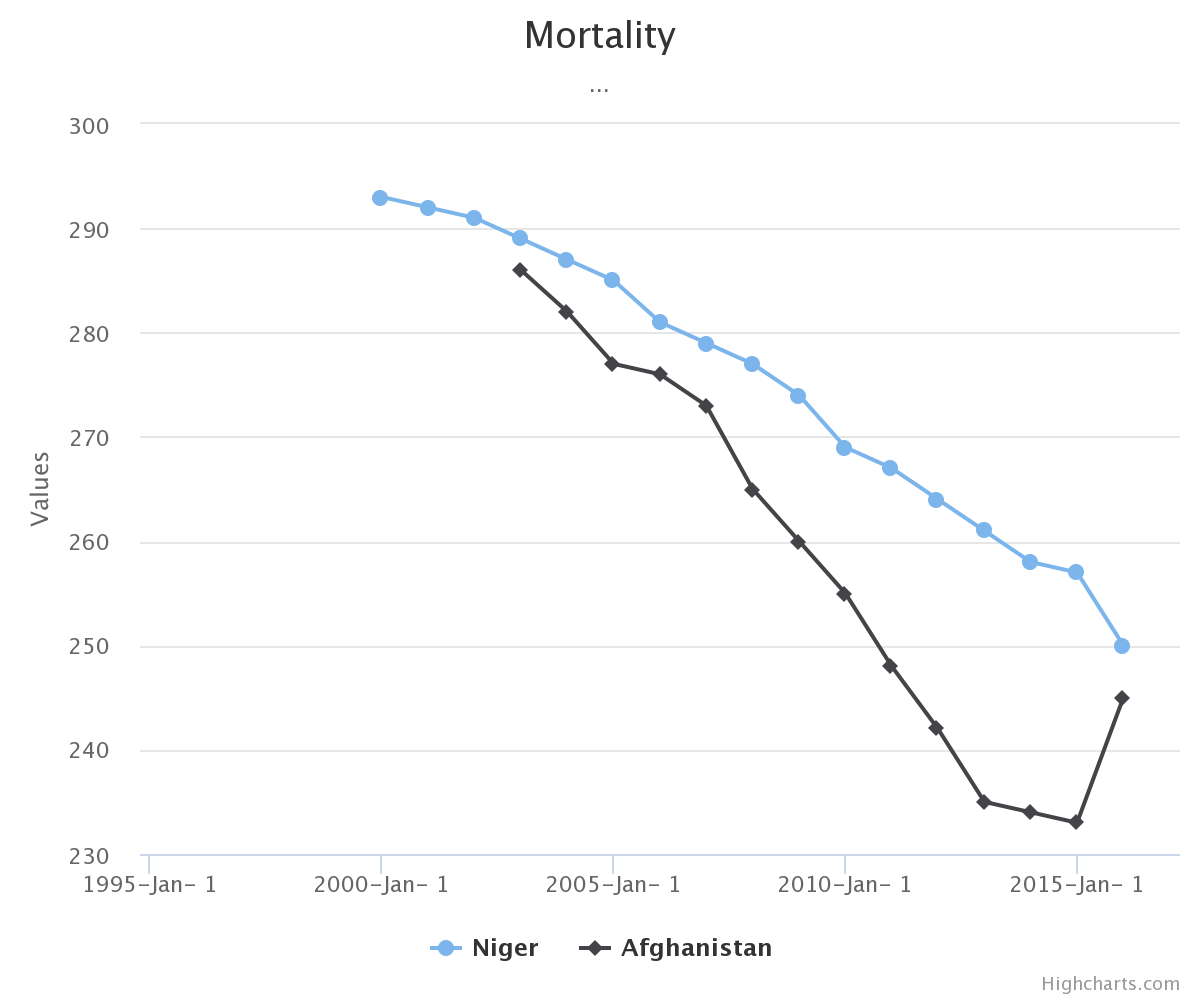
\includegraphics[scale=0.25]{images/mortality_rates_1.png}
    \caption{De sterftecijfers in Afghanistan en Niger in de periode van 2000 tot 2016.}
    \medskip
    \small
    %India, Pakistan en Nepal door het k-means algoritme geclassificeerd tot het cluster met relatief goedkopere graanprijzen.  
    \label{fig_sterfte}
    \end{figure}

\begin{figure}[h!]
        
        \centering
        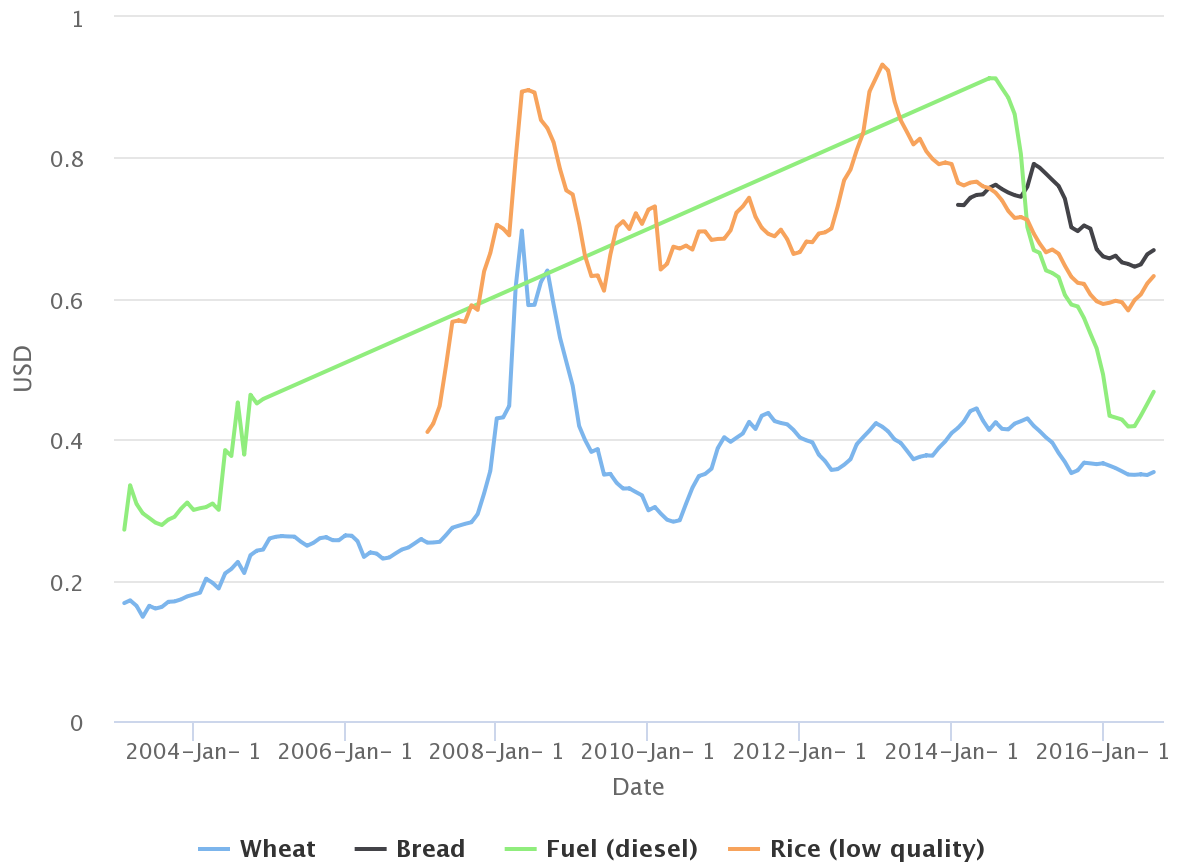
\includegraphics[scale=0.25]{images/mortality_product_afghanistan.png}
        \caption{De voedselprijzen in Afghanistan in de periode van 2004 tot 2016.}
        \medskip
        \small
        %India, Pakistan en Nepal door het k-means algoritme geclassificeerd tot het cluster met relatief goedkopere graanprijzen.  
        \label{mortality_afghanistan}
        \end{figure}



 \begin{figure}[h!]
        \centering
        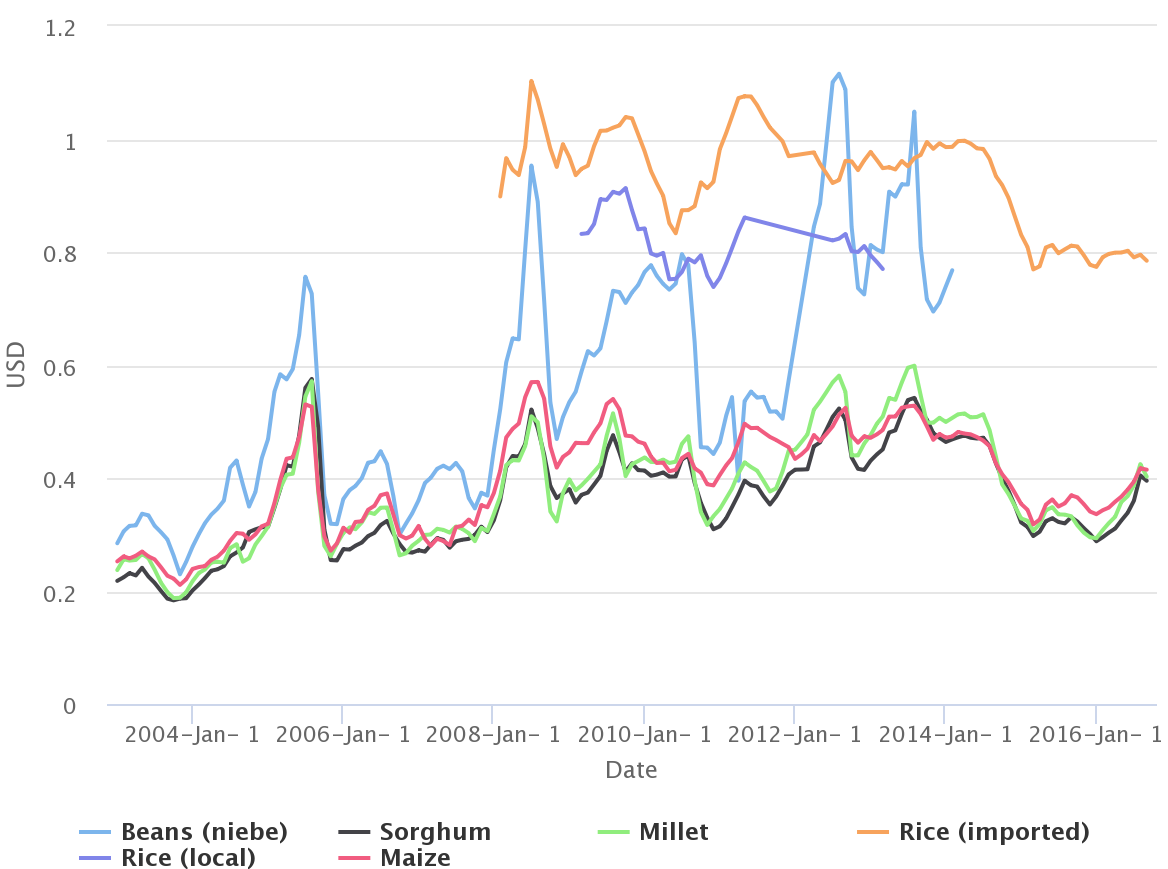
\includegraphics[scale=0.27]{images/mortality_product_niger.png}
        \caption{De voedselprijzen in Niger in de periode van 2004 tot 2016.}
        \label{mortality_niger}
        \medskip
        \small
        %India, Pakistan en Nepal door het k-means algoritme geclassificeerd tot het cluster met relatief goedkopere graanprijzen.  
        \end{figure}






\newpage
\subsubsection*{Bestaat er een verband tussen vluchtelingen-stromingen en voedselprijzen?}

Uit figuur \ref{fig_ref_afg} blijkt een grote stijging in het aantal vluchtelingen vanuit Afghanistan rond 2016. In Georgia vindt die grote stijging rond 2010 plaats (zie figuur\ref{fig_ref_geor}). Alle voedselprijzen in Afghanistan laten rond 2016 juist een daling zien (zie figuur \ref{mortality_afghanistan}). Ook de voedselprijzen in Georgia dalen of blijven stabiel rond 2010  (zie figuur \ref{georgia}). De gemiddelde correlatie van de voedselprijzen in Afghanistan en de vluchtelingen tussen 2015 en 2017 is -0.20. Voor Georgia is dat  -0.22.


\begin{figure}[h!]
    \centering
    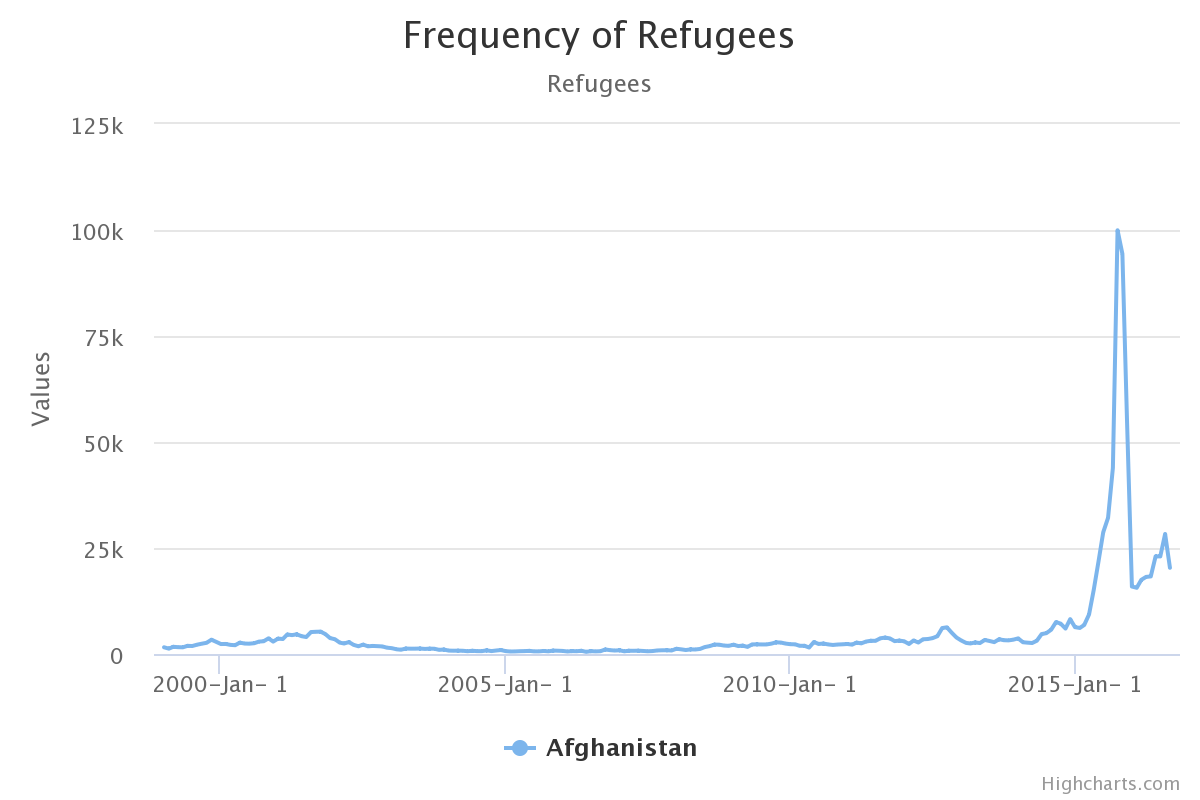
\includegraphics[scale=0.3]{images/refugees_1.png}
    \caption{Het aantal vluchtelingen van Afghanistan in de periode tussen 2000 en 2016 }
    \label{fig_ref_afg}
    \medskip
    \small
    %India, Pakistan en Nepal door het k-means algoritme geclassificeerd tot het cluster met relatief goedkopere graanprijzen. 
    \end{figure}

\begin{figure}[h!]
        \centering
        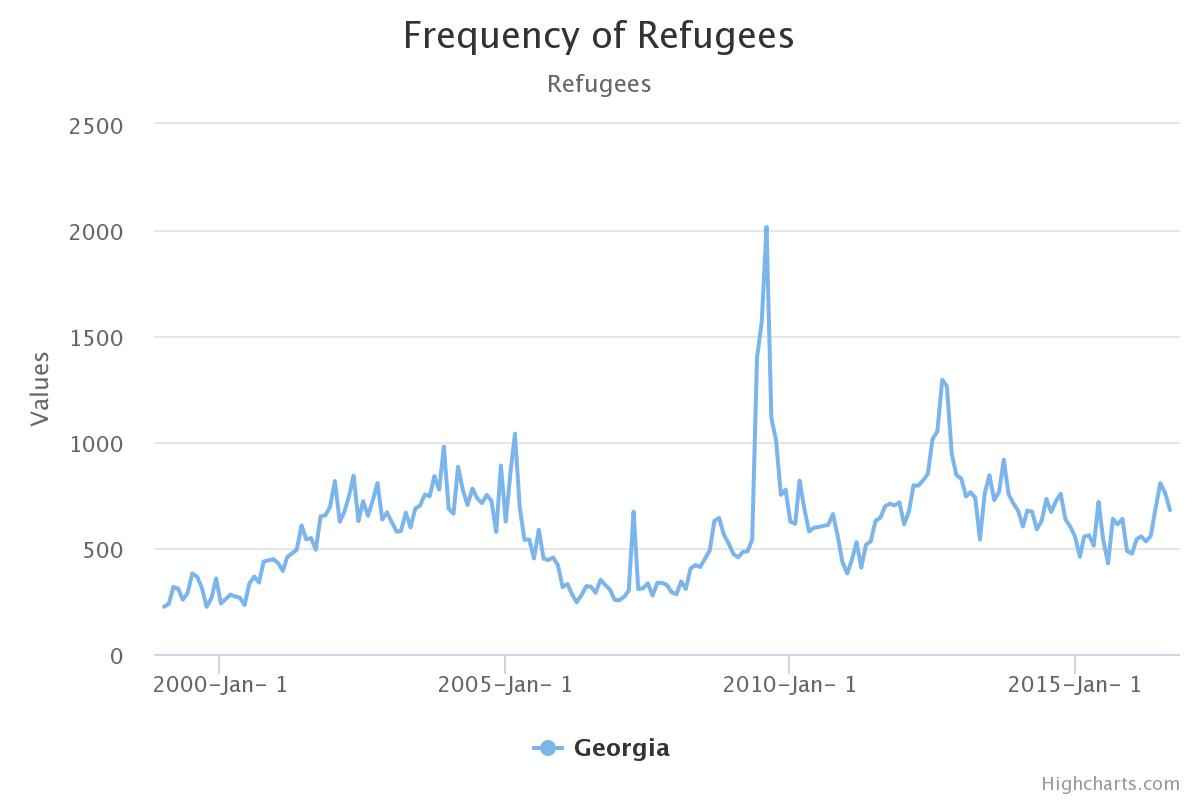
\includegraphics[scale=0.28]{images/refugees_georgia.jpeg}
        \caption{Het aantal vluchtelingen van Georgië in de periode tussen 2000 en 2016}
        \medskip
        \small
        %India, Pakistan en Nepal door het k-means algoritme geclassificeerd tot het cluster met relatief goedkopere graanprijzen. 
        \label{fig_ref_geor}
        \end{figure}


 \begin{figure}[h!]
        \centering
        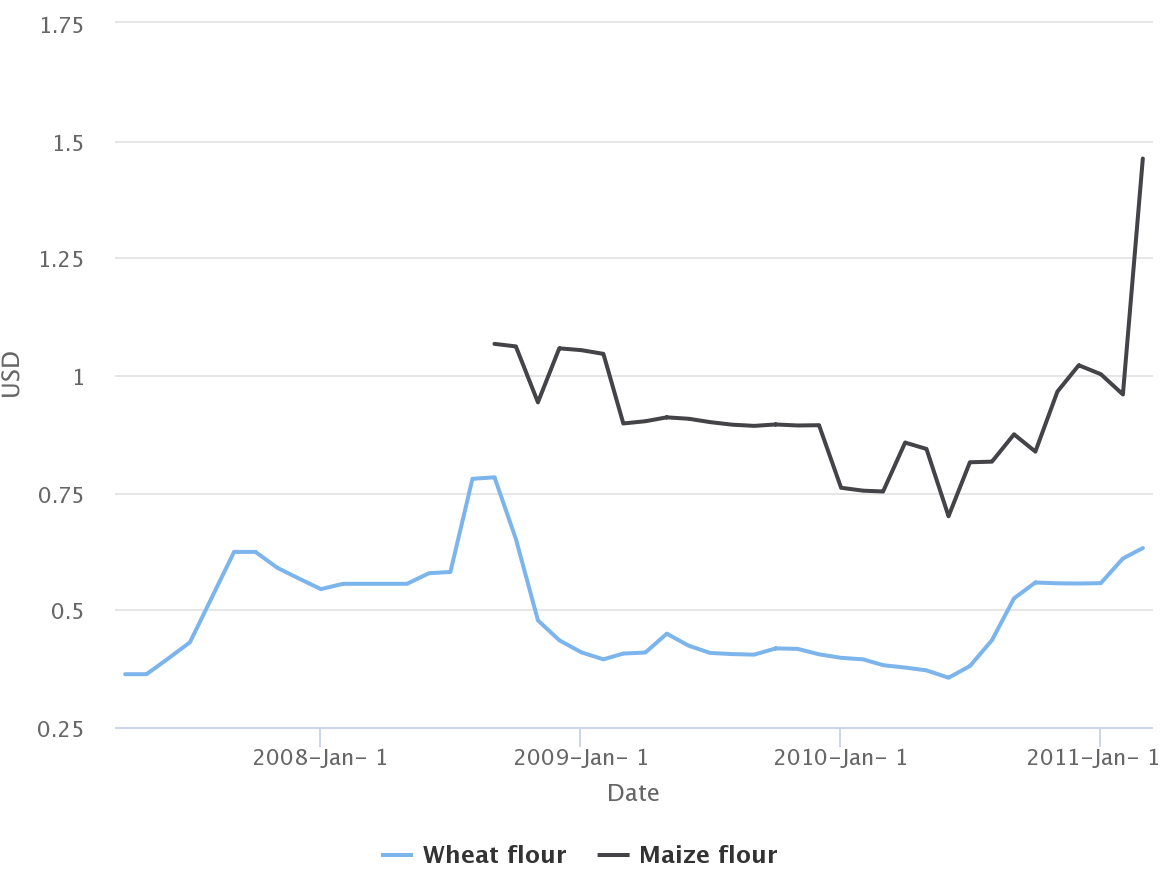
\includegraphics[scale=0.25]{images/Georgia.png}
        \caption{De voedselprijzen in Georgië in de periode tussen 2008 en 2011}
        \medskip
        \small
        %India, Pakistan en Nepal door het k-means algoritme geclassificeerd tot het cluster met relatief goedkopere graanprijzen. 
        \label{georgia}
        \end{figure}
        
\newpage
\section*{Discussie}

\subsubsection*{Vertonen landen in dezelfde regio’s vergelijkbare prijsverschillen?}
Dat het gebruik van k-means niet tot vaste cluster-groepen leidt, kan betekenen dat er sprake is van één cluster.
Ook als er naar de grafieken \ref{rice-regio} en \ref{sorghum-regio} wordt gekeken kan dit verklaard worden. De prijzen van de verschillende landen vertonen immers allemaal soortgelijke fluctuaties, waardoor k-means waarschijnlijk niet tot consistente classificaties kan komen.
Dit is in overeenstemming met de verwachting, omdat het allemaal landen binnen één regio betreft.
De relatief lage correlaties van Ethiopië, Liberia en Nigeria betekent mogelijk dat het \textit{outliers} zijn. Dat het k-means algoritme ook deze drie landen samen met de andere landen clustert, desondanks dat ze afwijken, kan verklaard worden doordat k-means geen \textit{outliers} kan detecteren.

 
% k-means geeft als resultaat dat er een verband is tussen vrijwel alle prijzen van rijst van de landen in Sub-Saharan Africa omdat er niet sprake is van consistente clustering. Dat wil zeggen dat het niet mogelijk is om meerdere groepen te vormen omdat de landen als het ware één grote groep vormen. 
% De lineaire correlatie tussen Ethiopia en Nigeria met de andere landen is aanzienlijk laag. Dit is niet gevonden met k-means omdat dit algoritme geen \textit{outliers} kan detecteren of het kan zijn dat de relatie is niet lineair is. De rijst prijzen van andere landen in Sub-Saharan Africa correleren wel sterk. \\
% Bij het bekijken van de prijzen van kafferkoor valt op dat er een subgroep ontstaat van Burkino-Faso, Mali en Niger tegenover de rest van de landen in \textit{Sub-Saharan Africa}. Met behulp van de correlatie coëfficiënten valt op dat er een hoge correlatie is tussen de prijzen van kafferkoor in landen Mali en Niger, Mali en Burkina Faso, en Niger en Burkina Faso. Dit laat zien dat landen in dezelfde regio's vergelijkbare prijsverschillen vertonen. 


\subsubsection*{Zijn er voedselprijzen die positief of negatief aan elkaar gecorreleerd zijn? Als voedselprijzen aan elkaar gecorreleerd zijn, is dit dan altijd het geval of alleen tijdens bepaalde periodes?}
Zoals uit figuur \ref{clusters-2013-2018} blijkt, worden vleesproducten altijd binnen één groep geclusterd en zuivelproducten ook. Dit is in overeenstemming met de verwachting, omdat dit twee verschillende voedsel-categorieën zijn. De hoge correlaties binnen deze clusters bevestigt ook het vermoeden dat producten uit dezelfde categorie soortgelijke prijsfluctuaties laten zien. Dat het vijfde cluster uit willekeurige producten lijkt te bestaan, komt waarschijnlijk door toevallige correlatie tussen de prijzen van deze producten. Dat \textit{sunflower oil} samen met brood wordt geclassificeerd kan verklaard worden doordat dat mogelijk een veelgebruikt ingrediënt voor brood is, maar ook dit kan door toeval worden verklaard.
Tot slot blijkt het kijken naar verschillende periodes vrijwel dezelfde correlaties op te leveren, wat het vermoeden bevestigd dat de periode geen invloed heeft op prijs-correlaties. Om dit met zekerheid te zeggen, zijn echter vergelijkingen over langere periodes nodig.


% Tabel 2 geeft de hoge correlaties weer tussen de verschillende vleessoorten in Oekraïne. %Dit kan verklaard worden aan de hand van: uitleg waarom 

% Zoals te zien is in Tabel 1 is de correlatie tussen de zuivel producten in Oekraïne tussen 2013 en 2018 zeer hoog. Bovendien worden deze producten bij elkaar geclusterd door k-means (zie tabel 3). Dit duidt dus op een positieve correlatie tussen de voedselprijzen van zuivelproducten (in Oekraïne). Deze correlatie was vooral te vinden in de periode tussen 2013 en 2018. 
%terug komen op hypothese

\subsubsection*{Zijn de wisselkoersen gecorreleerd aan de productprijzen in een land?}
Er blijkt een lichte correlatie (-0.283) te zijn tussen de wisselkoers en productprijzen. De grote standaardafwijking suggereert echter dat deze correlatie per product verschilt. Dit is in overeenstemming met de verwachting, aangezien de wisselkoers vooral invloed heeft op geïmporteerde producten. De grote standaardafwijking valt ook te verklaren doordat een productprijs doorgaans van veel factoren afhangt, waardoor de prijs soms sterker en soms zwakker lijkt te correleren met de wisselkoers. In het vervolg kan daarom onderscheid gemaakt worden tussen geïmporteerde en lokaal-geproduceerde producten, waarbij ook rekening wordt gehouden met andere factoren die van invloed zijn op de prijs van een product, zoals weersomstandigheden en transportkosten.




\subsubsection*{Geven prijzen gecorrigeerd op het Gross Domestic Product (GDP) een ander beeld dan prijzen in USD?}
Dat Nepal eerst tot het goedkopere graanprijs-cluster wordt gerekend, maar aan de hand van de betaalbaarheid-index tot een duurdere cluster, laat zien dat het gebruik van de betaalbaarheid-index een maatstaf is om in overweging te nemen. Waarschijnlijk geeft het vooral bij armere landen een betrouwbaarder beeld van de daadwerkelijke betaalbaarheid van producten, omdat het GDP in deze landen erg laag is. Bovendien blijkt er geen correlatie (-0.024) te zijn tussen GDP en productprijzen. Dit laat zien dat het GDP van een land  geen invloed heeft op de productprijzen van dat land, waardoor de betaalbaarheid-index als zuivere maat kan worden gebruikt. 
Echter zegt de betaalbaarheid van een product nog niet alles over toegang tot dat product. Daarom kan in vervolgonderzoek de betaalbaarheid-index gecombineerd worden met de beschikbaarheid van producten om zo een beeld te geven van de voedselzekerheid in een land.


\subsubsection*{Bestaat er een verband tussen de voedselprijzen en het sterftecijfer in een land?}
Er is geen duidelijk verband te vinden tussen de voedselprijzen en het sterftecijfer in Afghanistan en Niger.
Dit kan verklaard worden doordat wanneer de voedselprijzen stijgen, mensen waarschijnlijk over zullen gaan op andere, goedkopere voedselproducten om in leven te blijven. Daarnaast zijn er mogelijk andere factoren die het sterftecijfer sterk beïnvloeden, zoals natuurrampen, waardoor de invloed van voedselprijzen op het sterftecijfer niet is terug te zien in de data. In vervolgonderzoek zou daarom gekeken kunnen worden of de consumptie van relatief goedkope producten stijgt wanneer voedselprijzen stijgen, en of er andere factoren aanwezig zijn die het sterftecijfer kunnen beïnvloeden. De lichte correlaties die gevonden zijn tussen de voedselprijzen en sterftecijfers in beide landen zijn waarschijnlijk het resultaat van toeval.



\subsubsection*{Bestaat er een verband tussen vluchtelingen-stromingen en voedselprijzen?}
Er is geen duidelijk verband te vinden tussen de vluchtelingen-stromingen en de voedselprijzen in Georgia en Afghanistan. 
Dit kan verklaard worden doordat emigreren vaak lange tijd kost, waardoor stijgingen van voedselprijzen misschien pas later worden gevolgd door toenames van vluchtelingen stromingen. Zo stijgt de prijs van rijst in Afghanistan tussen 2013 en 2014 aanzienlijk (zie figuur \ref{mortality_afghanistan}) en stijgt het aantal vluchtelingen vanuit Afghanistan sterk vanaf 2015 (zie figuur \ref{fig_ref_afg}). Bovendien kunnen er mogelijk andere factoren zijn die de vluchtelingen stromingen sterk beïnvloeden, zoals oorlogen, waardoor de invloed van voedselprijzen op de vluchtelingen stromingen niet terug te zien is in de data. Tot slot is geen sterke correlatie gevonden tussen beide cijfers.


% De zwakke negatieve correlatie coëfficiënten kunnen verklaard worden aan de hand van twee mogelijkheden. De eerste optie is dat het verband te klein is om uit de data af te leiden. Dit zou kunnen zijn omdat in de figuren \ref{refugees_1} en \ref{mortality_afghanistan} en in de figuren \ref{refugees_georgia} en \ref{georgia} te zien is dat wanneer er een toename is in de voedselprijs er ook een toename is in het aantal vluchtelingen. Dit hoeft niet meteen te betekenen dat er een direct verband is tussen de twee fenomenen. Het kan ook zijn dat ze door een overeenkomstige factor worden beïnvloed. De tweede optie is dat er simpelweg geen correlatie aanwezig is tussen de vluchtelingen-stromen en voedselprijzen en dat de pieken in de grafieken toevallig samenvallen.  

\newpage

\printbibliography


\end{document}
